\section{An�lise de ilumina��o ambiente}
%http://www.princeton.edu/~achaney/tmve/wiki100k/docs/Photoresistor.html
%http://www.resistorguide.com/photoresistor/
\cite{CHEN201649}
Sensores de luminosidade servem para indicar a intensidade da luz que est� sendo aplicada ao ambiente controlado. Sua medi��o � feita mensurando a quantidade de energia radiante existente em uma das faixas de frequ�ncias da luz, podendo ser sens�vel a Luz vis�vel aos humanos, IR ou UV \figurename{wavelengthlight}. 

\begin{figure}[tbh!]
	\centering
	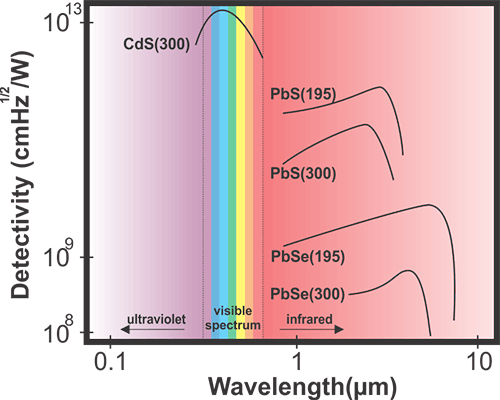
\includegraphics[width=1.0\textwidth]{../images/wavelength-detectivity}
	\caption{Faixas de luz capturadas por cada tipo de sensor}
	\label{fig:wavelengthlight}
\end{figure}

Os sensores de luminosidade s�o componentes eletr�nicos passivos do tipo resistor vari�vel, cuja resist�ncia varia dependendo da intensidade de luz recebida (nos spectros vis�veis ou IR). 

Esses componentes podem ser agrupados em 2 categorias principais: Os que respondem aos est�mulos de luz gerando energia el�trica (ex: fotovoltaico ou fotoemissivo) e os que respondem alterando suas pr�prias propriedades el�tricas (ex: fotoresistor ou fotocondutor). Sendo os fotoresistores (ex: LDR) mais utilizados para simples an�lise do n�vel de luminosidade, devido ao seu reduzido custo.


\acronym{IR}{Infra vermelho} 
\acronym{UV}{Ultravioleta}
\acronym{PbS}{Lead sulfide}
\acronym{PbSe}{lead selenide}
\acronym{InSb}{Indium antimonide}
\acronym{CdS}{Cadmium sulfide}
\acronym{CdSe}{Cadmium selenide}
\acronym{Ge:Cu}{Germanium cooper}
\acronym{LDR}{Light-Dependent Resistor}
\acronym{PLS}{Photovoltaic light sensors}
\acronym{PD}{Photo diode}